\subsection{Power measurement}
To look at the energy consumption in detail, the N6705B power analyzer from keysight was used as the power supply.
To carry out measurements, the ADP5090 with the solar cells and super cap was disconnected and the remaining components connected to the power analyser with a fixed voltage of 3.3\,V.
This way, the voltage and current over one write-cycle could be tracked.
The result is plotted in Figure \ref{results:ui}.
\begin{figure}[ht]
	\centering
	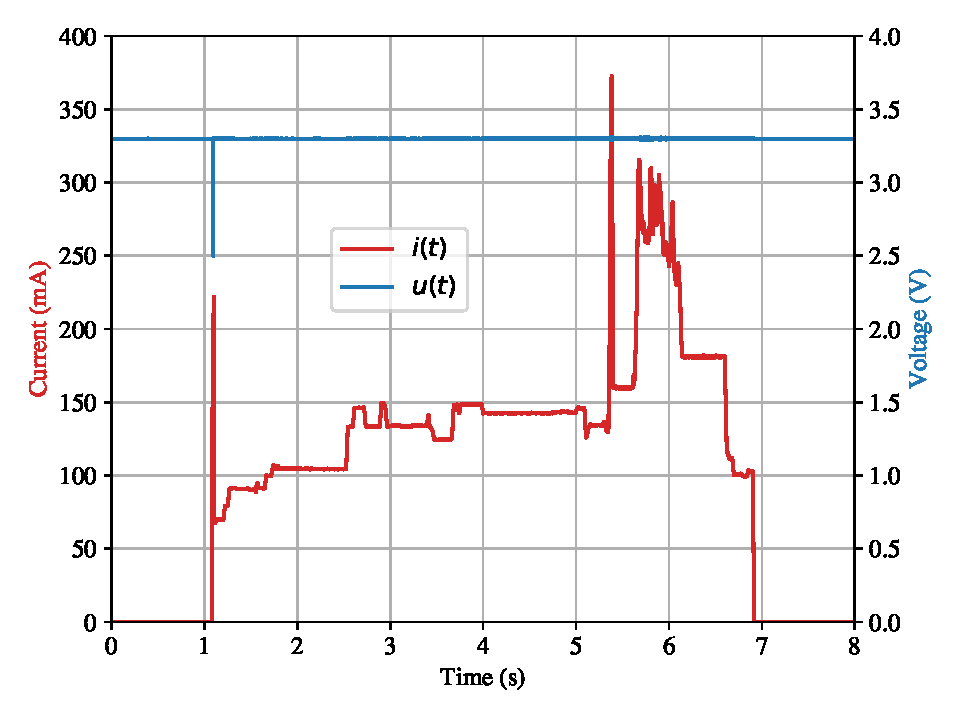
\includegraphics[width=0.9\textwidth]{5-results/energy/logger/ui.pdf}
	\caption{Current and Voltage during one write-cycle.\label{results:ui}}
\end{figure}
One write-cycle takes about 5.8 seconds.
In this interval, the STM32, nRF52480 and display driver are active.
Clearly visible is the current peak which occurs when the system is woken up.
Short after the 5 seconds mark, initializing and data receiving is finished and the display is refreshed.
The current peaks there are due to the charge pumps on the display driver.

With voltage and current given, the power over time can be calculated.
This curve is plotted in Figure \ref{results:p}.
The power follows obviously the same course like the current since the voltage is constant.
\begin{figure}[ht]
	\centering
	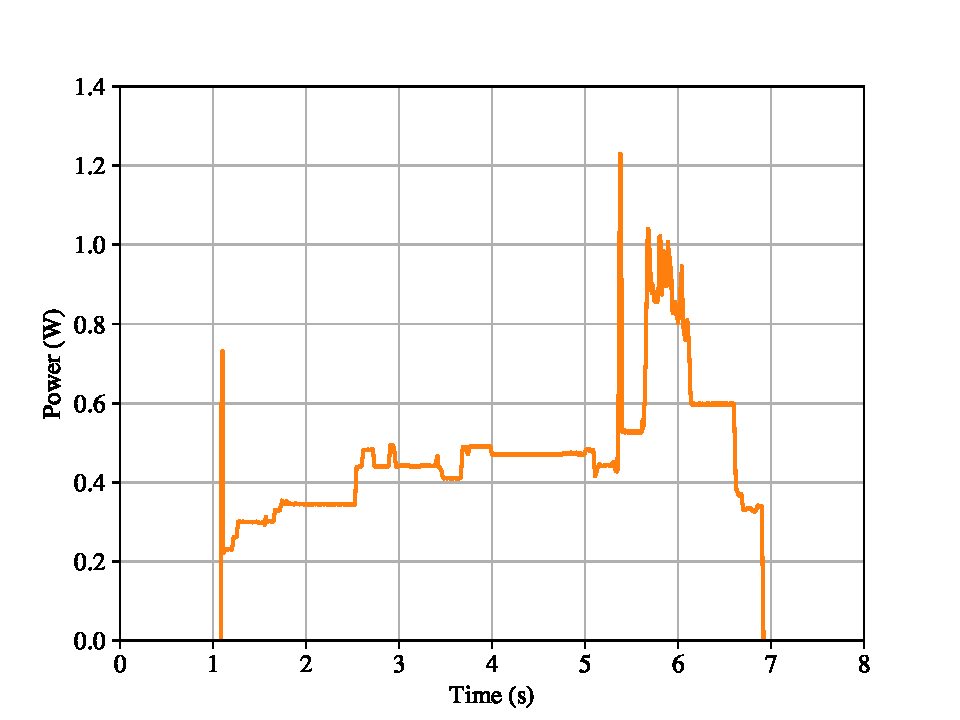
\includegraphics[width=0.9\textwidth]{5-results/energy/logger/p.pdf}
	\caption{Power consumption during one write cycle.\label{results:p}}
\end{figure}
The energy needed for one write-cycle is given with the integral of the power over time:
\begin{align}
	E = \int_{0}^{8\,\text{s}}P(t)\text{dt}\approx 2.7504\,\text{J}.
\end{align}
Like stated in \eqref{development:cell_power} the solar cells provide $485.52\,\mu \text{W}$ at 200\,lux.
Considering the Rficient which consumes $4.5\mu \text{W}$, it is possible to estimate the time needed, to harvest the power for one write cycle:
\begin{align}
	t_{\text{E}}=\frac{2.7504\,\text{J}}{485.52\,\mu \text{W}-4.5\mu \text{W}}=5717.85\,\text{s}\approx 1\,\text{h } 35\,\text{min}.
\end{align}
Not taken into account is the leakage of the super capacitor and losses in the ADP5090.

\subsection{Energy storage}
The stored energy in a capacitor is
\begin{align*}
	E =\frac{1}{2}CU^2.
\end{align*}
since the capacitor operates between 2.2\,V and 3.6\,V, the total stored energy is
\begin{align}
	E_{\text{ges}} = \frac{1}{2}C(U_{\text{max}}^2-U_{\text{min}}^2)=\frac{1}{2}\cdot 40\,\text {F}\cdot((3.6\,\text{V})^2-(2.2\,\text{V})^2)=162.4\,\text{J}.
\end{align}
If again the loss in the ADP5090 and the leakage of the super cap is neglected, it is possible to estimate the time
\begin{align}
	t_{\text{func}}=\frac{162.4\,\text{J}-2.7504\,\text{J}}{4.5\,\mu\text{W}}=3.54877\cdot 10^{-7}\,\text{s}\approx 411\,\text{d}
\end{align} 
in which the prototype is fully functional when no energy is harvested.
The 2.7504\,J are subtracted, because on should be able to refresh the display after this time.
This result should be taken with caution, because it neglects losses and does not consider the tolerance of the capacitor ($\pm20\%$ corresponds to $\pm8\,\text{F}$ with a 40\,F capacitor \cite{yuden}).
The order of magnitude tough should be correct.
